\newpage
\section{Centralised Controller}\label{sec:mpicontroller}

To facilitate communication between nodes using the hardware interface, we introduce a centralised controller. The centralised controller works by gathering requests (broadcasting, listening, or sleeping) from all nodes and processing these. The pseudo code description of the controller can be seen in \autoref{algo:mpicontroller}.\medbreak

The controller works by continuously awaiting requests from any of the nodes in the network on \autoref{line:action-await}. A call of any of the hardware functions described in \autoref{sec:mpiprotocol} will result in a message arriving at the controller. Whenever a message has been received, the controller will update the local time of the sending node in the nodes variable on \autoref{line:action-updatelocaltime}. We keep track of the currently known local times for all nodes in order to know when we are ready to process listen requests. \smallbreak

If the request is a transmit request (\autoref{line:action-transmit}), we add the request to the transmissions list, to be processed later. Should the request be a listen request (\autoref{line:action-listen}), we instead add a request to the listens list. Note that any call to the \texttt{Sleep} or \texttt{ReportLocalTime} functions are handled at \autoref{line:action-updatelocaltime}.\smallbreak

After processing the message, we compute the minimum local time of all the nodes stored in the nodes variable on \autoref{line:controllertime}. The controllertime is used to check whether we are ready to process any of the listen requests stored in the listens variable. We iterate through these on \autoref{line:iterlistens} and check if the end of the listen interval is greater than the minimum local time computed earlier. If this is the case, or if the listen request has already been processed, we continue iterating through the list. Otherwise, we begin iterating each transmission request stored in the transmissions list on \autoref{line:itertransmissions}, and if the transmission interval is within the current listen interval (\autoref{line:iswithin}), we check if the packet should be received by the listening node by calling the \texttt{ShouldReceive} function, and if yes, we add the packet to the list of packets to be sent to the listening node. We send the packets to the listening node on \autoref{line:sendpackets}.\medbreak

The \texttt{ShouldReceive} function (\autoref{algo:controllershouldreceive}) contains a pseudo code description of how we can use the packet error probability function from \autoref{sec:pep}, and defines the set of transmissions happening at the same moment ($nodes_t$). \medbreak


\begin{algorithm}[ht]
    \DontPrintSemicolon
    \KwResult{True if the transmission should be received.}
    \SetKwFunction{FShouldReceive}{ShouldReceive}
    \SetKwProg{Fn}{Function}{}{}
    
    \Fn{\FShouldReceive{l, t, transmissions, packetsize}}{
        $n_r \leftarrow$ l.id\;
        $n_t \leftarrow$ t.id\;
        $nodes_t \leftarrow$ empty Transmission list\;

        \ForEach{t$^\prime$ $\in$ transmissions - \{t\}}{
            \If{t.end $>$ t$^\prime$.start \And t.start $<$ t$^\prime$.end}{
                \Append t$^\prime$ \To nodes$_t$\;
            }
        }

        probability $\leftarrow$ $P_p(\text{n}_r, \text{m}_t, \text{nodes}_t, \text{packetsize})$\;
        should-receive $\leftarrow$ randomly choose based on probability\;
        \KwRet should-receive\;
    }

    \caption{The \texttt{ShouldReceive} Function.}
    \label{algo:controllershouldreceive}
\end{algorithm}


\begin{algorithm}[H]
    \DontPrintSemicolon
    \SetKwFunction{FController}{Controller}
    \SetKwProg{Fn}{procedure}{}{}

    \textbf{Structure} Message \{ action, source, localtime, duration, data \}\;
    \textbf{Structure} Transmission \{ source, start, end, data \}\;
    \textbf{Structure} Listen \{ source, start, end \}\;
    \textbf{Structure} Node \{ localtime \}\; % location
    \;

    \Fn{\FController{}}{
        transmissions $\leftarrow$ empty Transmission list\;
        listens $\leftarrow$ empty Listen list\;
        nodes $\leftarrow$ map containing all nodes with id as key\;
        \;
        \Repeat{\textit{protocol terminates}}{
            m $\leftarrow$ \Await Message \From any node\; \label{line:action-await}
            nodes(m.source).localtime $\leftarrow$ m.localtime + m.duration\; \label{line:action-updatelocaltime}

            \If{m.action = transmit}{ \label{line:action-transmit}
                t $\leftarrow$ Transmission \{ m.source, m.localtime, m.localtime $+$ m.duration, m.data \}\;
                \Append t \KwTo transmissions\;
            }
            \ElseIf{m.action = listen}{ \label{line:action-listen}
                l $\leftarrow$ Listen \{ m.source, m.localtime, m.localtime $+$ m.duration \}\;
                \Append l \KwTo listens\;
            }

            controllertime $\leftarrow \min_{\forall \text{n} \in \text{nodes}}$(n.localtime)\; \label{line:controllertime}

            \ForEach{l $\in$ listens}{ \label{line:iterlistens}
                \If{l.end $>$ controllertime}{% \Or l.processed}{
                    \Continue
                }

                packets $\leftarrow$ empty Packet list\;

                \ForEach{t $\in$ transmissions}{ \label{line:itertransmissions}
                    \If{t.id $=$ l.id}{
                        \Continue
                    }

                    \If{t.start $\geq$ l.start \And t.end $\leq$ l.end}{ \label{line:iswithin}
                        \If{\texttt{ShouldReceive}(l, t, transmissions, |t.data|)}{ \label{line:shouldreceive}
                            \Append t.data \To packets\;
                        }
                    }
                }

                \Send $|$packets$|$ \To l.id\; \label{line:sendcount}

                \ForEach{p $\in$ packets}{ \label{line:sendpackets}
                    \Send p \To l.id\;
                }

                %l.processed $\leftarrow$ true\;
            }

            \ForEach{l $\in$ listens}{
                \If{controllertime $>$ l.end}{
                    \Remove l \From listens\;
                }
            }

            \ForEach{t $\in$ transmissions}{
                \If{controllertime $>$ t.end}{
                    \Remove t \From transmissions\;
                }
            }

        }
    }
    \caption{The \texttt{Controller} procedure.}
    \label{algo:mpicontroller}
\end{algorithm}

\begin{figure}[H]
    \centering
    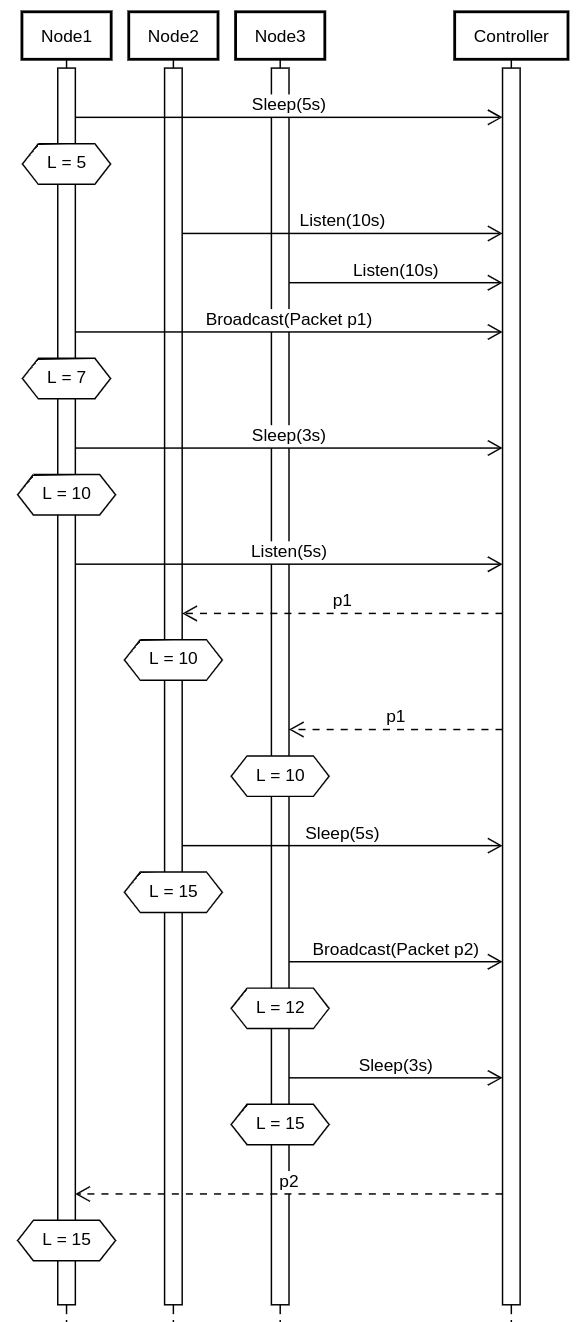
\includegraphics[width=0.6\textwidth]{figures/controller_sequence.png}
    \caption{A sequence diagram showing an example communication flow between three nodes and the controller.}
    \label{figure:mpi:controller:sequence-example}
\end{figure}

In \autoref{figure:mpi:controller:sequence-example}, we show a sample communication flow between three nodes and the centralised controller. The example is meant to show how the local time (L) of the nodes is continuously updated through the use of virtual time. For this example, we assume that a broadcast has a duration of two seconds, and the local time is initially $\text{L} = 0$. The figure demonstrates that whenever a node sleeps or broadcasts, the local time of the node is updated instantaneously, but when the node listens, its local time is updated only after receiving any packets transmitted within the listen interval. 






%The centralised controller consist of two concurrent procedures. The \texttt{MessageHandler} procedure (\autoref{algo:mpimessagehandler}), and the \texttt{Controller} procedure (\autoref{algo:mpicontrollerpart}). A shared state is used to manage the data between the two procedures (\autoref{algo:mpisharedstate}). \medbreak
%\todo[inline]{fix autoref for data structure}

%In essence, the centralised controller works by gathering all requests from all nodes in the \texttt{MessageHandler} procedure for a given time slot, and by processing, and responding to the requests in the \texttt{Controller} procedure.

% \begin{algorithm}[ht]
%     \DontPrintSemicolon
%     \SetAlgorithmName{Data Structure}{Data Structure}

%     \textbf{Structure} Message \{ action, source, localtime, duration, data \}\;
%     \textbf{Structure} Transmission \{ source, start, end, data \}\;
%     \textbf{Structure} Listen \{ source, start, end, processed \}\;
%     \textbf{Structure} Node \{ localtime \}\; % location
%     \;

%     queue $\leftarrow$ empty Message queue\;
%     transmissions $\leftarrow$ empty Transmission list\;
%     listens $\leftarrow$ empty Listen list\;

%     nodes $\leftarrow$ map containing all nodes with id as key\;
%     %transmissions $\leftarrow$ empty map\;

%     \caption{The shared state variables and structures used by the controller.}
%     \label{algo:mpisharedstate}
% \end{algorithm}

%The shared state consists of two structures, \texttt{Message} and \texttt{Node}, used to store messages and nodes respectively, as well as three global variables: \texttt{nodes}, \texttt{transmissions}, and \texttt{currenttime}. \smallbreak

%\texttt{nodes} is a map of key-value pairs, containing every node in the network, with the unique identifier of the node as the key, and a \texttt{Node} structure as the value. \smallbreak

%\texttt{transmissions} is another map of key-value pairs, where the key is the unique identifier of a transmitting node, and the value is the data packet sent from the node. \smallbreak

%\texttt{currenttime} is an integer used to keep track of the already processed time slots, whenever a time slot has been processed, this is incremented.

%\begin{algorithm}[ht]
%    \DontPrintSemicolon
%    \SetKwFunction{FMessageHandler}{MessageHandler}
%    \SetKwProg{Fn}{procedure}{}{}
%    
%    \Fn{\FMessageHandler{}}{
%        \Repeat{\textit{protocol terminates}}{
%            m $\leftarrow$ \Await Message \From any node\;
%        
%            \If{m.action = transmit}{
%                nodes(m.source).time $\leftarrow$ nodes(m.source).time + 1\;
%                nodes(m.source).state $\leftarrow$ transmitting\;
%                transmissions(m.source) $\leftarrow$ m.data\;
%            }
%            \ElseIf{m.action = listen}{
%                nodes(m.source).time $\leftarrow$ nodes(m.source).time + m.time\;
%                nodes(m.source).state $\leftarrow$ listening\;
%            }
%            \ElseIf{m.action = sleep}{
%                nodes(m.source).time $\leftarrow$ nodes(m.source).time + m.time\;
%                nodes(m.source).state $\leftarrow$ sleeping\;
%            }
%\ElseIf{m.action = location}{
%    nodes(m.source).location $\leftarrow$ m.data as location\;
%}
%        }
%    }
%    \caption{The MessageHandler procedure.}
%    \label{algo:mpimessagehandler}
%\end{algorithm}



%The task of the \texttt{MessageHandler} procedure is to continuously gather requests from all of the nodes in the network, and change the state and local time of the node in the \texttt{nodes} map, as well as storing the data packet for any transmitting node in the \texttt{packets} map. \medbreak

%Whenever requests have been gathered from all nodes for a time slot, we are able to process the time slot. This is the task of the \texttt{Controller} procedure. On \autoref{line:awaitprocess} in \autoref{algo:mpicontrollerpart}, we wait until every node in the \texttt{nodes} map has a $\texttt{time} > \texttt{currenttime}$, which means that every node has sent a request for the \texttt{currenttime}'th time slot. If this is the case, we are able to process the time slot. A time slot is processed by first iterating through all nodes that are either in the \texttt{transmitting} or \texttt{sleeping} state. If the node is transmitting, we need to distribute the packet to all neighbours of the node that are able to receive the packet, by adding the packet to the \texttt{packets} list in the \texttt{Node} structure. This is decided by the link model (TODO), where we compute the probability of the neighbour receiving the packet, as described in \autoref{sec:linkmodel}. Is the node currently sleeping, we send a wakeup message to the node, if the local time of the node is equal to our \texttt{currenttime} variable. \smallbreak

%\todo[inline]{Incorporate link model}

%After processing any transmitting or sleeping nodes, we iterate through the map of nodes once again, but this time we process any nodes currently listening for packets. If the local time of the node listening for packets is equal to our \texttt{currenttime} variable, we send any packets stored in the \texttt{packets} list of the node, and clear the contents of the list afterwards.

% \begin{algorithm}[ht]
%     \DontPrintSemicolon
%     \SetKwFunction{FProcessor}{Controller}
%     \SetKwProg{Fn}{procedure}{}{}

%     \Fn{\FProcessor{}}{
%         \Repeat{\textit{protocol terminates}}{
%             \Await every node $\in$ nodes, where node.time $>$ currenttime\;\label{line:awaitprocess}

%             currenttime $\leftarrow$ currenttime + 1\;

%             \ForEach{node $\in$ nodes}{
%                 \If{node.state = transmitting}{
%                     %m $\leftarrow$ Message\;
%                     %m.action $\leftarrow$ transmit\;
%                     data $\leftarrow$ transmissions(node.id)\;

%                     \ForEach{neighbour $\in$ neighbours(node)}{
%                         \If{neighbour.state = listening \And shouldreceive(neighbour)}{
%                             \Append data \KwTo neighbour.packets\;
%                         }
%                     }

%                     \Remove transmissions(node.id)\;
%                     \Send ack \KwTo node.id\;
%                 }
%                 \ElseIf{node.state = sleeping \And node.time = currenttime}{
%                     \Send wakeup \KwTo node.id\;
%                 }
%             }

%             \ForEach{node $\in$ nodes}{
%                 \If{node.state = listening \And node.time = currenttime}{
%                     \Send $|$node.packets$|$ \KwTo node.id\;                
%                     \ForEach{packet $\in$ node.packets}{
%                         \Send packet \KwTo node.id\;
%                     }

%                     \Clear node.packets\;
%                 }
%             }

%         }
%     }

%     \caption{The Controller procedure.}
%     \label{algo:mpicontrollerpart}
% \end{algorithm}
